
\documentclass[./thesis.tex]{subfiles}

 
\begin{document}


\alert{ Il faut ecrire quelque part la fonction d'onde:
$$ \ket{\Psi} = \sum_I^\Ndet c_I \kI $$
et l'expression des determinants:
\begin{equation}
\begin{array}{c}
 \Psi({\bf r}_1,\dots,{\bf r}_{\Na},{\bf r}_{\Na+1},\dots,{\bf r}_N;
      \alpha_1,\dots,\alpha_{\Na},\beta_{\Na+1},\dots,\beta_N) = \\
\left|
 \begin{array}{ccc}
 \varphi_1({\bf r}_1) & \dots & \varphi_1({\bf r}_{\Na}) \\
 \vdots               & \dots &   \vdots             \\
 \varphi_{\Na}({\bf r}_1) & \dots & \varphi_{\Na}({\bf r}_{\Na}) \\
 \end{array}
\right|
\left|
 \begin{array}{ccc}
 \varphi_1({\bf r}_{\Na+1}) & \dots & \varphi_1({\bf r}_{N}) \\
 \vdots               & \dots &   \vdots             \\
 \varphi_{N_\beta}({\bf r}_{\Na+1}) & \dots & \varphi_{N_\beta}({\bf r}_{N}) \\
 \end{array}
\right|
\end{array} 
\label{eq:slater}
\end{equation}
}

Generally speaking, implementing a wavefunction method requires iteration over either bielectronic integrals or determinants. \\
ease of implementation VS performances \\
ease of parallelism(?) \\
Need to explicitly maintain a list of determinant. \\




\section{Notation TBUpdated}
\begin{itemize}
	\item [$\Ne$] : Number of electrons.
	\item [$\Na$] : Number of $\alpha$-spin electrons.
	\item [$\Nb$] : Number of $\beta$-spin electrons.
	\item [$\Ndet$] : Number of determinants in the wavefunction.
	
	\item [$\Norb$] : Number of orbitals.

	\item [$\Nint$] : Number of 64-bit integers required to store $\Norb$ bits.
        $\Nint = \lfloor \frac{\Norb-1}{64} \rfloor + 1$
		
	\item [$\bitI$] : Bitstring representation of $\kI$
\begin{lstlisting}
integer*8 :: I(N_int, 2)
\end{lstlisting}
	
	\item [$\bitIsigma$] : 
	Bitstring representation of $\sigma$ spinorbitals of $\kI$, $\sigma \in \{\alpha, \beta\}$ 
\begin{lstlisting}
integer*8 :: Is(N_int)
\end{lstlisting}

	\item [ {$\bitIsigma [n] $} ] :
	Bitstring representation of $\sigma$ spinorbitals of $\kI$ in the range $[ 1+n \times 64, \min \qty (n \times 64 + 63, \Norb) ]$, $0 \leq n \leq \Nint-1 \; ;\; \sigma \in \{\alpha, \beta\}$
\begin{lstlisting}
integer*8 :: Isn
\end{lstlisting}

\end{itemize}

All the program is built such that the $\alpha$ and $\beta$ spinorbitals share the same space part. In other words, spinorbitals $i$ and $\bar{i}$ both refer to orbital $\phi_i(\br)$.


\section{Determinant internal representation}


Determinants can be written as a string of creation operators applying to the vacuum state $\vac$.
$$\ac{i} \ac{j} \ac{k} \vac = \kI$$
Because of the fermionic nature of electrons, permutation of two contiguous creation operators results in a sign change, which makes their ordering relevant.
$$\ac{j} \ac{i} = -\ac{i} \ac{j}$$
$$\ac{j} \ac{i} \ac{k} \vac = -\kI$$
This effectively allows to make any $\Nperm$ permutations (even of non-contiguous operators), and always get
$$-1^{\Nperm} \kI$$


We see a determinant can be broken down into two pieces of information:
\begin{itemize}
\item
An unordered set of creation operators. Essentially, the set of occupied spinorbitals.
\item
A sign, the so-called \emph{phase factor}, indicating whether the creation operators are ordered so as to refer to $\kI$ or $-\kI$.
\end{itemize}

Determinants are always associated with a coefficient, so we don't need to make the phase factor part of a determinant's internal representation ; the sign will simply be reported on the associated coefficient. Still, we have to make unambiguous to what exact determinant this coefficient applies to, so we need to define an ordering to which our ``phaseless'' representation implicitly refers. We choose the order where all the $\alpha$ spinorbitals are placed before the $\beta$ spinorbitals, and for each spin then orbitals are sorted with increasing indices.
For instance, the set of spinorbitals $\{\bar i, i,j,k \}$ with $j>i$ and $k>j$ refers to
$$\kJ = \ac{i} \ac{j} \ac{k} \ac{\bar i} \vac $$

So if we happen to build a determinant initially expressed as
$$\kJp = \ac{j} \ac{i} \ac{k} \ac{\bar i} \vac $$
It will be translated to $-\kJ$.


The occupations of the spinorbitals are stored using the so-called \emph{bitstring} encoding. A bitstring is an array of bits ; typically, the 64-bit binary representation of an integer is a bitstring of size 64.
Quite simply, the idea is to map each spinorbital to a single bit, whose value is set to its occupation number. In other words \texttt{0} and \texttt{1} are associated with the \emph{unoccupied} and \emph{occupied} states.
By this definition, bitstrings are essentially lists of occupation numbers, which is a convenient way to
store the set of occupied spinorbitals in a determinant.

For simplicity and performance considerations, the occupations of the $\alpha$ and $\beta$ spinorbitals are stored on different bitstrings, rather than interleaved or otherwise merged in the same one. This allows to straightforwardly map orbital index $n$ to bit index $n-1$ (orbitals are usually indexed from $1$, while bits are indexed from $0$), and makes a bitstring a set of orbitals.
This makes the representation of a determinant a tuple of two bitstrings, associated with respectively $\alpha$ and $\beta$ spinorbitals. Such objects are refered to as \emph{$\alpha \beta$-bitstrings}, and generally define a set a spinorbitals. When used to define a determinant, they imply the previously defined ordering.


\begin{itemize}
\item
$\bitI$ is the $\alpha \beta$-bitstring representation of $\kI$
\item
$\bitI_\alpha$ is the bitstring representation of the set of occupied $\alpha$ spinorbitals of $\kI$ 
\item
$\bitI_\beta$ is the bitstring representation of the set of occupied $\beta$ spinorbitals of $\kI$ 

\end{itemize}
%It's easier to think of $I_\alpha$ and $I_\beta$ as "sets of occupied $\alpha$/$\beta$ spinorbitals". But bitstrings are generally sets of orbitals, they are sets of spinorbitals only by context.
% C'est vrai dans RHF, pas dans UHF. Pas necessaire alors on peut virer la phrase.


The storage space required for a single determinant is, in principle, one bit per spinorbital, or $2 \times \Norb$ bits. However, because CPUs are designed to handle efficiently 64-bit integers, each spin part is stored as an array of 64-bit integers, the unused space being padded with zeros. 
The actual storage needed for a determinant is
$$
2 \times 64 \times  \left \lfloor \frac{\Norb-1}{64} + 1 \right \rfloor \, \text{bits}
\label{determinantstoragespace}
$$

For a given system, we call $\Nint$ the number of 64-bits integers needed to store one spin part.
\begin{equation}
\Nint = \left \lfloor \frac{\Norb-1}{64} \right \rfloor + 1
\end{equation}


The internal Fortran representation of a bitstring is an array of $\Nint$ \lstinline{integer*8}'s (64-bit integers).

The internal Fortran representation of an $\alpha \beta$-bitstring is a two dimensional array of \lstinline{integer*8}'s, the first dimension of size $\Nint$ and the second of size $2$, corresponding to the $\alpha$ and $\beta$ spin parts.


\lstset{frame=single}
\begin{lstlisting}
  ! I is an ab-bitstring
  ! I_alpha and I_beta are bitstrings
  
  integer*8 :: I(N_int, 2)
  integer*8 :: I_alpha(N_int), I_beta(N_int)

  ... ! load some determinant in I
  I_alpha(:) = I(:,1)
  I_beta (:) = I(:,2)
\end{lstlisting}
\lstset{frame=none}


In formulas or algorithms, depending on the level of detail desired, a bitstring can be treated as a single integer of infinite size. This hides some implementation details but is unambiguous. However, in algorithms we will usually try to stay closer to the actual implementation. $\bitI$ being the $\alpha \beta$-bitstring associated with $\kI$, we can explicitly refer to a single 64-bit integer
$$\bitI_{\sigma}[i]\; ;\; \sigma \in \{\alpha, \beta\}\; ;\; i \in [0, \Nint-1]$$
which is the bitstring representation of the $\sigma$ spinorbitals of determinant $\kI$ in the range $[1+i \times 64, \min \left( (i+1) \times 64, \Norb \right)]$, indexed from $0$ to $63$.

      
\section{Bit manipulation}

The bitstring encoding is a compact way of storing determinants, but it is more than just a storage method. It allows to perform a variety of operations on determinants by taking advantage of CPU's hardware aptitude to perform efficiently bitwise operations on integers.

In many of the presented algorithms, some Fortran intrinsics will be of use. Each of those maps to a CPU instruction that is available on modern CPUs.
%POPCNT, in particular, is a relatively recent instruction, and is standard starting from Fortran 2008.

%The pseudo-instruction
%\begin{lstlisting}
%assert LOGICAL_EXPRESSION
%\end{lstlisting}
%means \texttt{LOGICAL\_EXPRESSION} is guaranteed to be true. The syntax is otherwise Fortran-style.

      

\begin{sloppypar}
\begin{itemize}
	      
	\item $\POPCNT{\bitI}$ :
	Returns the number of non-zero bits for a given integer $\bitI$. \\
        ${\POPCNT{\binary{00011000}} = 2}$.
	      
	\item $\TRAILZ{\bitI}$ : Returns the number of trailing zero bits for a given integer \bitI. \\
         ${\TRAILZ{\binary{00000100}} = 2}$.
	      
	      
	\item $\IBCLR{\bitI}{n}$ : Returns the value of $\bitI$ with the bit at the $n$-th position set to zero (the rightmost bit is at position zero). \\
        ${\IBCLR{\binary{00001111}}{2} = \binary{00001011}}$.
	      
	     
   	\item $\IOR{\bitI}{\bitJ}$ : Bitwise \texttt{OR} logical operation. \\
        ${\IOR{\binary{1100}}{\binary{1010}} = \binary{1110}}$.

	 
	\item $\IEOR{\bitI}{\bitJ}$ : Bitwise \texttt{XOR} (exclusive or) logical operation. \\
        ${\IEOR{\binary{1100}}{\binary{1010}} = \binary{0110}}$.
	      
	      
	\item $\IAND{\bitI}{\bitJ}$ : Bitwise \texttt{AND} logical operation. \\
        ${\IAND{\binary{1100}}{\binary{1010}} = \binary{1000}}$.
	      
	      
	\item $\NOT{\bitI}$ : Bitwise \texttt{NOT} logical operation. \\
        ${\NOT{\binary{00001100}} = \binary{11110011}}$.
	      
	\item $\ISHFT{\bitI}{n}$ : Returns $\bitI$ with bits shifted $|n|$ places to the left if $n>0$, otherwise to right. Bits shifted out of the range are lost. Zeros are shifted from the opposite end. \\
        ${\ISHFT{\binary{01001110}}{2} = \binary{00111000}}$, \\
        ${\ISHFT{\binary{01001110}}{-2} = \binary{00010011}}$.
	      
	\item $\BTEST{\bitI}{n}$ : Returns $\TRUE$ if the $n$-th bit of $\bitI$ is set, otherwise $\FALSE$. \\
        $\BTEST{\binary{00001000}}{3} = \TRUE$.
	      
\end{itemize}
\end{sloppypar}
      
      
Those intrinsics apply to integers at most 64-bits. This however is a purely implementational limitation, so depending on the level of detail desired, this constraint can be unambiguously lifted in formulas or algorithms. Different notations will be used for the 64-bit and the infinite size cases, as they are not always equivalent.
For example, the 64-bit bit-shift intrinsic always returns zero for shifts greater than 64 bits:

$$ \ISHFT{1}{n} =
\begin{cases}
2^{n}, & 0 \le n < 64 \\
0, & \text{otherwise}
\end{cases}
$$

More convenient notations are also desired for some operators. All binary operators are of same precedence and left-associative.

\begin{table}[H]
	\begin{tabularx}{\textwidth}{X|X}
		\hline
		
		\hline
		\rule{0pt}{3ex}
		$\ISHFT{\bitI}{n}$ & $\ishft{I}{n}$  \\ 
		
		\hline
		\rule{0pt}{3ex}
		$\TRAILZ{\bitI}$ & $\trailz{I}$  \\ 
		
		\hline
		\rule{0pt}{3ex}
		$\IBCLR{\bitI}{n}$ & $\ibclr{I}{n}$  \\ 
		
		\hline
		\rule{0pt}{3ex}
		$\BTEST{\bitI}{n}$ & $\btest{I}{n}$  \\ 
		
		\hline
		\rule{0pt}{3ex}
		$\NOT{\bitI}$ & $\neg I $  \\ 
		
		\hline
		\rule{0pt}{3ex}
		$\IAND{\bitI}{\bitJ}$ & $\iand{I}{J}$ \\
		
		\hline
		\rule{0pt}{3ex}
		$\IOR{\bitI}{\bitJ}$ & $\ior{I}{J}$ \\
		
		\hline
		\rule{0pt}{3ex}
		$\IEOR{\bitI}{\bitJ}$ & $\ieor{I}{J}$ \\
		
		\hline
		\rule{0pt}{3ex}
		$\POPCNT{\bitI}$ & $\popcnt{I}$ \\
		\hline
	\end{tabularx}
\end{table}

Note that these notations apply to integers ; whether or not they are meant to be bitstrings.



       
Some examples of how these instructions can be used are given below. They are key to understand how we can determine which holes and particles are created when exciting from $\kI$ to $\kJ$.
Let $\bitI$ and $\bitJ$ be the bitstring representations of $\kI$ and $\kJ$, and $\bit{P}$ a bitstring with $\Nint=1$. 


%TODO : Confusion entre sets et integers
%TODO : Confusion entre sets et integers en dessous. Introduire notation curly pour les sets
      
      
\begin{itemize}
	      
	\item
		$I_{\alpha}$ : the set of orbitals containing an $\alpha$ electron in $\ket I$
	            
	\item
		$|I_{\alpha}|$ : number of orbitals in the set $I_{\alpha}$. In other words, number of $\alpha$ electrons in $\ket I$ 
	            
	\item
		$I_{\alpha} \oplus J_{\alpha}$ : set of $\alpha$ spinorbitals that are contained in exactly one of $I_{\alpha}$ or $J_{\alpha}$. In other words, $\alpha$ spinorbitals whose occupation status change when exciting between $\ket I$ and $\ket J$. 
	            
	\item
		$|I_{\alpha} \oplus J_{\alpha}|/2$ : half the number of $\alpha$ spinorbitals whose occupation status changes when exciting between $\ket I$ and $\ket J$. Because an excitation means a status change for exactly 2 spinorbitals, this value is the $\alpha$ excitation degree between $\ket I$ and $\ket J$.
	            
	\item
		$(I_{\alpha} \oplus J_{\alpha}) \wedge J_{\alpha}$ :
		%$iand(J_{\alpha}, ieor(I_{\alpha}, J_{\alpha}))$ :
	      The set of $\alpha$ spinorbitals that are occupied in $\ket J$ and whose occupation status changes when exciting between $\ket I$ and $\ket J$. In other words, the set of $\alpha$ spinorbitals where particles are created when exciting from $\ket I$ to $\ket J$ or where holes are created when exciting from $\ket J$ to $\ket I$.
	            
	\item
		$TRAILZ(P)+1$ :
	      If $P$ is the empty set, returns $65$. Otherwise returns the index of the lowest orbital in set $P$.
	            
	\item
		$IBCLR(P,TRAILZ(P))$ :
	      if $P$ is the empty set, the empty set. Otherwise, the set $P$ minus its orbital of lowest index.
\end{itemize}


\section{Computing Excitations}

An algorithm used to compute excitation degree is presented as algorithm \ref{alg:EXC_DEGREE}, and one to compute the sets of created holes and particles as algorithm \ref{alg:EXC}. Algorithm \ref{alg:EXC}, however, returns the sets as determinants bitstrings. Extracting the indices from a bitstring is another basic operation, presented as algorithm \ref{alg:LIST_FROM_BITSTRING}.
Because computing excitations is done heavily, and because we are typically interested in double excitations at most, a more specialized algorithm can be used ( PAS ENCORE ECRIT/POMPÉ )


\begin{algorithm}[h!]
	\caption{EXC\_DEGREE}
	\label{alg:EXC_DEGREE}
	\SetKwFunction{FMain}{EXC\_DEGREE}
	\SetKwProg{Fn}{Function}{:}{}
	
	\Fn(\tcc*[h]{Computes the excitation degree between two determinants}){\FMain{$I, J$}}{
		\KwData {$I, J$ bitstring representations of determinants $\ket I$ and $\ket J$}
		\KwResult{ Returns the excitation degree between $\ket I$ and $\ket J$ }

		$X \gets 0$   \;
		\For{$\sigma \in \{\alpha, \beta\}$}{
		\For{$i \gets 0, \Nint-1$}{
		  $X \gets X+POPCNT(IEOR(I_{\sigma}[i], J_{\sigma}[i]))$  \;
		}
		}
		\KwRet $X / 2$\;
	}
\end{algorithm}


\begin{algorithm}[H]
	\caption{EXC}
		
	\SetKwFunction{FMain}{EXC}
	\label{alg:EXC}
	\SetKwProg{Fn}{Function}{:}{}
	
	\Fn(\tcc*[h]{Returns the holes and particles created in an excitation, as bitstrings}){\FMain{$I$,$J$}}{
	\KwData{ $I, J$ bitstring representations of determinants $\ket I$ and $\ket J = \hat T \ket I$}
	\KwResult{ Returns a tuple $(P,H)$, $P$ and $H$ are respectively the sets of particles and holes created by $\hat T$, as $\alpha \beta$-bitstrings}
		\For{$\sigma \in \{\alpha, \beta\}$}{
		\For{$i \gets 0, \Nint-1$}{
			$C \gets IEOR(I_{\sigma}[i],  J_{\sigma}[i])$\;
			$P_{\sigma}[i] \gets IAND(C, J_{\sigma}[i])$\;
			$H_{\sigma}[i] \gets IAND(C, I_{\sigma}[i])$\;
		}
		}
		\KwRet{ $(P,H)$}\;
		}
\end{algorithm}




\begin{algorithm}[h!]
	\caption{LIST\_FROM\_BITSTRING}
	\label{alg:LIST_FROM_BITSTRING}
	\SetKwFunction{FMain}{LIST\_FROM\_BITSTRING}
	\SetKwProg{Fn}{Function}{:}{}
	
	\Fn(\tcc*[h]{Returns the indices contained in a bitstring as a list of integers}){\FMain{$P$}}{
		\KwData{ $P$ a bitstring }
		\KwResult{ $L$ the list of indicies contained in $P$ in increasing order. $P$ is destroyed. }
		$k \gets 0$ \;
		\For{$i \gets 0, \Nint-1$}{
		\While{$P[i] \neq 0$}{
		$e \gets TRAILZ(P[i])$\;
		$P[i] \gets IBCLR(P[i], e)$\;
		$L[k] \gets e + i \times 64$\;
	    $k \gets k+1$\;
		}
		}
		\KwRet{$L$}
		}
		
\end{algorithm}



\section{Computing phase factors}



A bit more complex is the computation of phase factors. The following explaination is limited to one spin part. More details will be given about why spin parts can be treated independently.
As we have seen in chapter XXXX, our $\alpha \beta$-bitstring representation of determinants has an implied ordering for creation operators : sorted first by spin $\alpha$ before $\beta$, then by increasing orbital index.
Whenever we build a new determinant by applying an excitation operator, we get a determinant that is initially expressed not just with a different ordering, but with a mix of creation and anihilation operators.

In most cases, permuting contiguous operators will still just result in a sign change.

$$a_j a_i = -a_i a_j$$
$$a^\dagger_j a^i = -a_i a^\dagger_j ; i \neq j$$
$$a^\dagger_i a_i = 1-a_i a^\dagger_i$$

The special case is the permutation of a creation and an anihilation in the same spinorbital. Indeed

$$a_l a^\dagger_l \ket I  = \ket I ; a^\dagger_l a_l \ket I = 0 ; l \notin \{i,j,k\}$$

In the first case, a particle is created then anihilated, resulting in the same determinant. In the second case, there is an attempt at anihilating a particle that does not exist, resulting in $0$. This is of course reversed if $l \in \{i,j,k\}$.

$$a_l a^\dagger_l \ket J  = 0 ; a^\dagger_l a_l \ket J  = \ket J; l \in \{i,j,k\}$$


Equations ( les deux dernieres ) allow to remove anihilation operators from the expression of a determinant.



Single excitation operators are defined as

$$\hat T_j^l=a^\dagger_l a_j$$

Be $\ket I$ and $\ket K$ two determinants directly representable as $\alpha \beta$-bitstrings, $i<j<k<l$.

$$\ket I = a^\dagger_i a^\dagger_j a^\dagger_k \ket \ $$
$$\ket K = a^\dagger_i a^\dagger_k a^\dagger_l \ket \  $$


What happens if we apply the excitation operator $\hat T_j^l=a^\dagger_l a_j$ to $\ket I$?


$$\hat T_j^l \ket I = a^\dagger_l a_j a^\dagger_i a^\dagger_j a^\dagger_k \ket \ $$

We now have to re-order the operators to get something representable as a bitstring, by permuting contiguous operators. It takes $n=1$ permutation to bring $a^\dagger_j$ in front of $a_j$.


$$\hat T_j^l \ket I = -a^\dagger_l a_j a^\dagger_j a^\dagger_i a^\dagger_k \ket \ $$

Using equation (plus haut)

$$\hat T_j^l \ket I = -a^\dagger_l a^\dagger_i a^\dagger_k \ket \ $$

Then, it takes $n$ permutations to bring $a^\dagger_l$ to the position formerly occupied by $a^\dagger_j$, and $x=1$ more permutation to bring it at its final position.

$$\hat T_j^l \ket I = -a^\dagger_i a^\dagger_k a^\dagger_l \ket \  = -\ket K$$

The total number of permutations needed is $2n+x$. The parity of the number or permutations is the parity of $x$. As can be seen, $x$ is the number of particles between spinorbitals $j$ and $l$ in $\ket I$ ( regardless of whether $l>j$ or $l<j$ ). In our case, there was 1 occupied spinorbital $k$, so the number of needed permutation is odd, so we ended with a negative phase factor.

\begin{figure}[h!]
	\begin{center}
		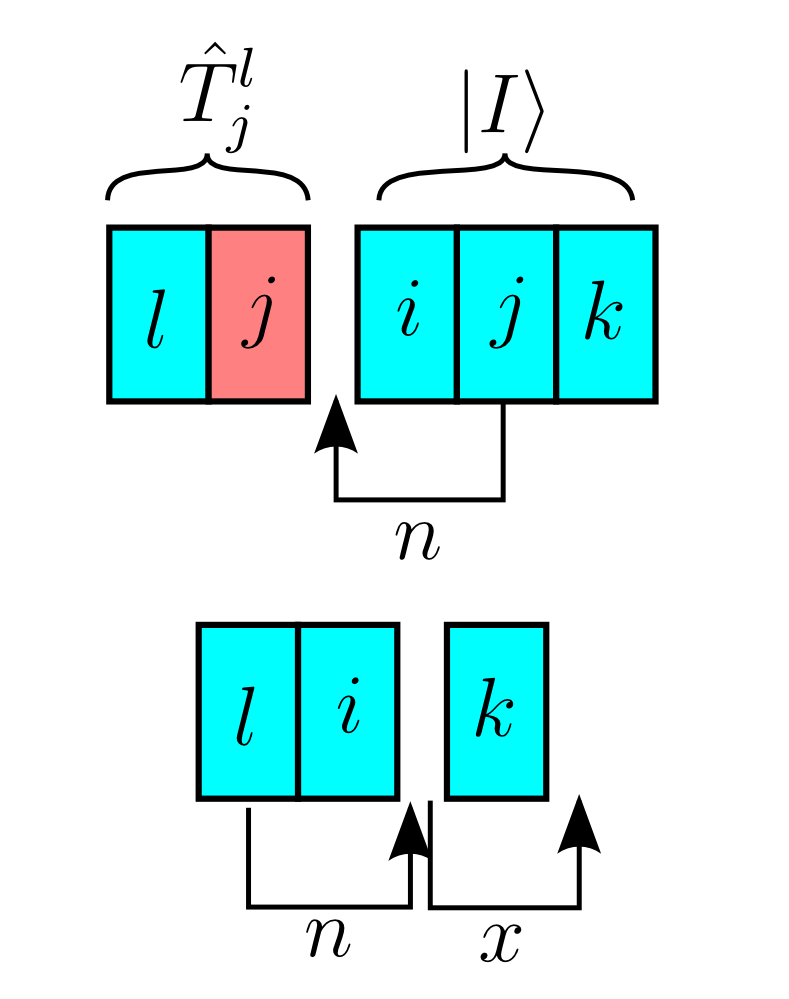
\includegraphics[width=0.3\columnwidth]{figures/determinant_driven/phasefactor}
		\caption{
		\label{phasefactor}%
		phasefactor
		}
		commentt
	\end{center}
\end{figure}

\subsection{Treating spin parts separately}

It is not immediately obvious that $\alpha$ and $\beta$ spin parts can be treated independently. We can do it because we chose to sort creation operators firstly by spin.

Be $\hat D_\alpha^I$ the serie of creation operators that creates all $\alpha$ electrons for $\ket I$ by increasing orbital indices, and $\hat D_\beta^I$ the operator that creates all $\beta$ ones.

$$\ket I = \hat D_\alpha^I \hat D_\beta^I \ket \ $$


$\ket I$ is representable as an $\alpha \beta$ bitstring. Be $\hat T_\alpha$ and $\hat T_\beta$ excitation operators of any degree that only involve $\alpha$ or $\beta$ spinorbitals, respectively.

$$\hat T_\alpha \hat T_\beta \ket I = \ket J = \hat T_\alpha \hat D_\alpha^I \hat T_\beta D_\beta^I \ket \ = \pm \hat D_\alpha^J \times \pm \hat D_\beta^J \ket \ $$

with

$$\hat D_\alpha^J = \pm \hat T_\alpha \hat D_\alpha^I$$
$$\hat D_\beta^J = \pm \hat T_\beta \hat D_\beta^I$$

As can be seen, the phase factor will be computed by independentely re-ordering $\hat T_\alpha \hat D_\alpha^I$ and $\hat T_\beta \hat D_\beta^I$.

We could move $\hat T_\beta$ inbetween $D_\alpha^I$ and $D_\beta^I$, because this will always be done in an even number of permutations, and thus will not result in a sign change. Because $\hat T_\beta$ is an excitation operator, it involves as many creations as anihilations, and moving together an even number of operators results in an even number of permutations. We are guaranteed never to encounter the special case of permuting $a^\dagger_i$ with $a_i$ because of the different spins.






A phase factor depends on an excitation operator $\hat T$ and a determinant $\ket S$ it is applied to. We always assume $\hat T \ket S \neq 0$ with $\hat T$ at most a biexcitation. 



\subsection{Monoexcitation}

%In the case of a monoexcitation, only one spin part is involved. All indices refer to spinorbitals of same, arbitrary spin $\sigma \in \{\alpha, \beta\}$

For a given determinant $\ket S$ and $\ket{\alpha}=a^\dagger_{j'} a_{i'}  \ket S$, the phase factor of the matrix element $\Hij{S}{\alpha}$ can be determined by the parity of
$$N^{S}_{ij}=\sum_{i<k<j} occ^{S}_{k};i=min(i',j');j=max(i',j')$$
With $occ^{S}_{k}$ the occupation number of spinorbital $k$ for $\ket S$ or $\ket \alpha$. Note that occupation numbers in $\ket S$ and $\ket \alpha$ are by construction equal for any spinorbital $k \neq i \neq j$, so while we will use $\ket S$ in the following, we could as well use $\ket \alpha$. This is obvious from the fact that $\Hij{S}{\alpha}=\Hij{\alpha}{S}$  

Parity of an integer $X$ can be defined by $$p(X)=X \wedge 1$$
        
Indeed $p(X)=0$ if and only if X is even, $p(X)=1$ if and only if X is odd. $p(X)$ is of the same parity as $X$, so 
$$-1^{N_{perm}} = -1^{p(N_{perm})}$$
        
        

A bitstring $R_{ij}$, containing all orbitals in a given range $]i, j>i[$ can be built as follow
$$R_{ij}=ishft(not(0),i) \oplus ishft(not(0),j-1)$$


Be $S$ the bitstring reprensentation of $\ket S$, $N^{S}_{ij}$ The number of $\sigma$ electrons for $\ket S$ in the given orbital range can be evaluated as
$$N^{S}_{ij} = |S_\sigma \wedge R_{ij}|$$

Thus 

$$phase(ij, \ket S) = -1^{p(N^S_{ij})}$$
Using the above formulas and taking into account the bitstring's internal representation as arrays of integer*8 size $\Nint$, we get algorithm \ref{alg:PHASE_MONO}.   


\begin{algorithm}
	\caption{PHASE\_MONO}	
	\label{alg:PHASE_MONO}
				\SetKwFunction{FMain}{PHASE\_MONO}
	\SetKwProg{Fn}{Function}{:}{}
	
	\Fn(\tcc*[h]{Compute phase factor of $\Hij{I}{I_a^b}$}){\FMain{$I_\sigma, a, b$}}{
		\KwData{ $I_\sigma$ the bitstring representation of $\sigma \in \{\alpha, \beta\}$ spinorbitals of $\ket I$}
		\KwData{ $a,b$ indices of a hole and a particle created in $\sigma$ spinorbitals of $\ket I$ }
		\KwResult{ The phase factor associated with $\Hij{I}{I_a^b}$}
		$high \gets max(a,b)-1$ \;
		$low \gets min(a,b)-1$ \;
		$il \gets \frac{low}{64} + 1$ \;
		$ih \gets \frac{high}{64} + 1$ \;
		$l \gets mod(low, 64)$ \;
		$h \gets mod(high, 64)$ \; 
		\For{$i \gets il, ih-1$}{
			$mask[i] = NOT(0)$\;		
		}

		%$mask[ih] \gets ISHFT(NOT(0), h-63)$ \;
		%$mask[il] \gets IAND(mask[il], ISHFT(NOT(0), l))$ \;
		
		$mask[ih] \gets ISHFT(NOT(0), h+1)$ \;
		$mask[il] \gets IEOR(mask[il], ISHFT(NOT(0), l))$ \;
		
		
		$nperm \gets 0$ \;
		\For{$i \gets il,ih$}{
			$nperm \gets nperm + POPCNT(IAND(I_{i}, mask[i]))$ \;
		}
		}
\end{algorithm}
        

\subsection{Phasemasks}


Algorithm \ref{alg:PHASE_MONO} is a general one, efficient for computing the phase factor for two arbitrary determinants. However, a phase computation is typically needed every time an integral is accessed, resulting in a vast amount of computational power being consumed. When only this method was used in the quantum package, it wasn't uncommon to find that most computational power was used on phase computations.
Advantage can be taken of the fact that, in most cases, the considered determinants aren't actually arbitrary. Usually, phase computation will be performed repeatedly on a same determinant, or on determinants of the wavefunction. For a fairly modest computational price, it is possible to compress the phase information from a particular determinant and make it cheaper to extract. The underlying principle is little more than a cumulative sum. If, for a determinant $\ket S$ that is going to be used repeatedely for phase computation, we pre-compute
        
$$E^S_{i} = \sum_{k < i} occ^{S}_{k}$$
        
We can access $N^S_{ij}$ for any $i$ and $j>i$ with no need to loop over $occ^{S}_{k}$

$$\tilde N^S_{ij} = E^S_j - E^S_{i+1} ; i \neq j$$
$$N^S_{ij} = \tilde N^S_{ij} ; j>i$$

Note that $\tilde N^S_{ij}$ is still defined when $j<i$. The reason for this will be made clear later.
This requires to store $E^S$ which is an integer array of size $2 \times (\Norb+1)$. Note that there is a slight waste as $E^S_1 = 0 \forall \ket S$ ( there is always $0$ electrons under the first orbital ) and $E^S_{\Norb+1} = N_{electron,\sigma} \forall \ket S$ ( there is always $N_{electron,\sigma}$ electrons in all orbitals ). Those values are still stored for convenience.






\begin{comment}
This requires to store $E^S$ which is an integer array of size $2 \times (\Norb+1)$.
Note that although only $2 \times \Norb$ integers are required to store the whole information, for practical reasons the actual size of the array is $2 \times (\Norb+1)$ because when the last orbital is involved, we need to access $E_{\Norb+1}$. The reason for this loss is that $E_1$ contains no information - there are always 0 electrons under the first orbital, $E^S_1 = 0 \forall \ket S$.
\end{comment}

This may be somewhat memory consuming if we want to pre-compute and store $E$ for each determinant. However, because the actual information needed isn't $N^S_{ij}$, but merely its parity, we only need to store the so-called "phasemask" vector $P^S$

$$P^S_i = p(E^S_i)$$

which is 1 bit of information per spinorbital, as opposed to an integer big enough to accomodate a number of electrons.
       
$$E^S_i = 2 \times  \lfloor \frac{E^S_i}2 \rfloor + P^S_i$$
$$\tilde N^S_{ij} = E^S_j - E^S_{i+1} = 2 \times \big ( \lfloor \frac{E^S_j}2 \rfloor - \lfloor \frac{E^S_{i+1}}2 \rfloor \big ) + P^S_j - P^S_{i+1}$$
	    
In the last equation, $\tilde N^S_{ij}$ is expressed as a sum of 3 terms. The first one being even by construction, the parity of $\tilde N^S_{ij}$ is the parity of the rest of the sum.
$$p(\tilde N^S_{ij})=p(P^S_j - P^S_{i+1})$$
This can be rewritten in a slightly more efficent way as
$$p(\tilde N^S_{ij}) = P^S_j \oplus P^S_{i+1}$$

Note that using $E^S$ instead of $P^S$ would require an extra ADD instruction ( totalement negligeable ? )
$$p(\tilde N^S_{ij}) = (E^S_{i+1} - E^S_j) \wedge 1$$

We have used sorted indices $i<j$. But just like for the general algorithm, if we consider $\hat T_{i'}^{j'}$, it looks like we need to sort $i'$ and $j'$ to get the $i$ and $j$ indices used for phase computation.

$$i=min(i', j') ; j=max(i', j')$$

This however doesn't need to be done explicitely. We can arbitrarily choose $i=i'$ and $j=j'$, and reverse the phase if $j<i$. We effectively have computed $p(N^S_{i'j'})$ instead of $p(N^S_{j'i'})$, and it can be proven they are always of diffrent parity.

$$\tilde N^{S}_{i' j'} + \tilde N^{S}_{j'i'} = E^{S}_{j'} - E^S_{i'+1} + E^S_{i'} - E^S_{j'+1} = -(occ^S_{j'} + occ^S_{i'})$$

Because $\hat T_{i'}^{j'} \ket S \neq 0$, we know that $occ^S_{j'} + occ^S_{i'} = 1$. 

$$\tilde N^{S}_{j' i'} = -(\tilde N^{S}_{i'j'} + 1)$$

This translates to $\tilde N^{S}_{j' i'}$ and $\tilde N^{S}_{i'j'}$ being of different parity.



\begin{algorithm}
	\caption{PHASEMASK}	
	\label{alg:PHASEMASK}	
	\SetKwFunction{FMain}{PHASEMASK}
	\SetKwProg{Fn}{Function}{:}{}
	
	\Fn(\tcc*[h]{Compute a phasemask}){\FMain{$I$}}{
		\KwData{ $I$ the bitstring representation of $\ket I$}
		\KwResult{ $P$ is the phasemask vector associated with $\ket I$, as described in section XXXXX}
		   
		\For{$\sigma \in \{\alpha, \beta\}$}{
		 $p \gets 0$ \;
		\For{$i \gets 0, \Nint-1$}{
		 $n \gets min(64, \Norb - i \times 64)$ \;
		\For{$j \gets 0,n-1$}{
		 $P_\sigma[i \times 64 + j] \gets p$ \;
		\If{$BTEST(I, j)$}{
		 $p \gets IEOR(p, 1)$ \;
		%\Comment flips the first bit
		}
		}
		}
		 $P_\sigma [\Norb] \gets p$ \;
		}
		\KwRet{$P$} \;
		}
\end{algorithm}

\begin{algorithm}
	\caption{PHASE\_FROM\_PHASEMASK}	
	\label{alg:PHASE_FROM_PHASEMASK}	
	\SetKwFunction{FMain}{PHASE\_FROM\_PHASEMASK}
	\SetKwProg{Fn}{Function}{:}{}
	
	\Fn(\tcc*[h]{Compute phase from phasemask}){\FMain{$P^I$, $i$, $j$}}{
		\KwData{ $P^I$ is the phasemask vector associated with $\ket I$, as described in section XXXXX. $i$ and $j$ spinorbitals of spin $\sigma \in \{\alpha, \beta \}$ so that $\hat T_i^j \ket I \neq 0 $}
		\KwResult{ The phase factor of  $\Hij{I}{a_i a^\dagger_j \ket I}$.}

		\uIf{$j < i$}{
			$c \gets 1$ \;
		}
		\Else{
			$c \gets 0$ \;		
		}
		\KwRet{$-1^{(c \oplus P^I_\sigma[i+1] \oplus P^I_\sigma[j])}$} \;
		}
\end{algorithm}

                
\begin{figure}[h!]
	\begin{center}
		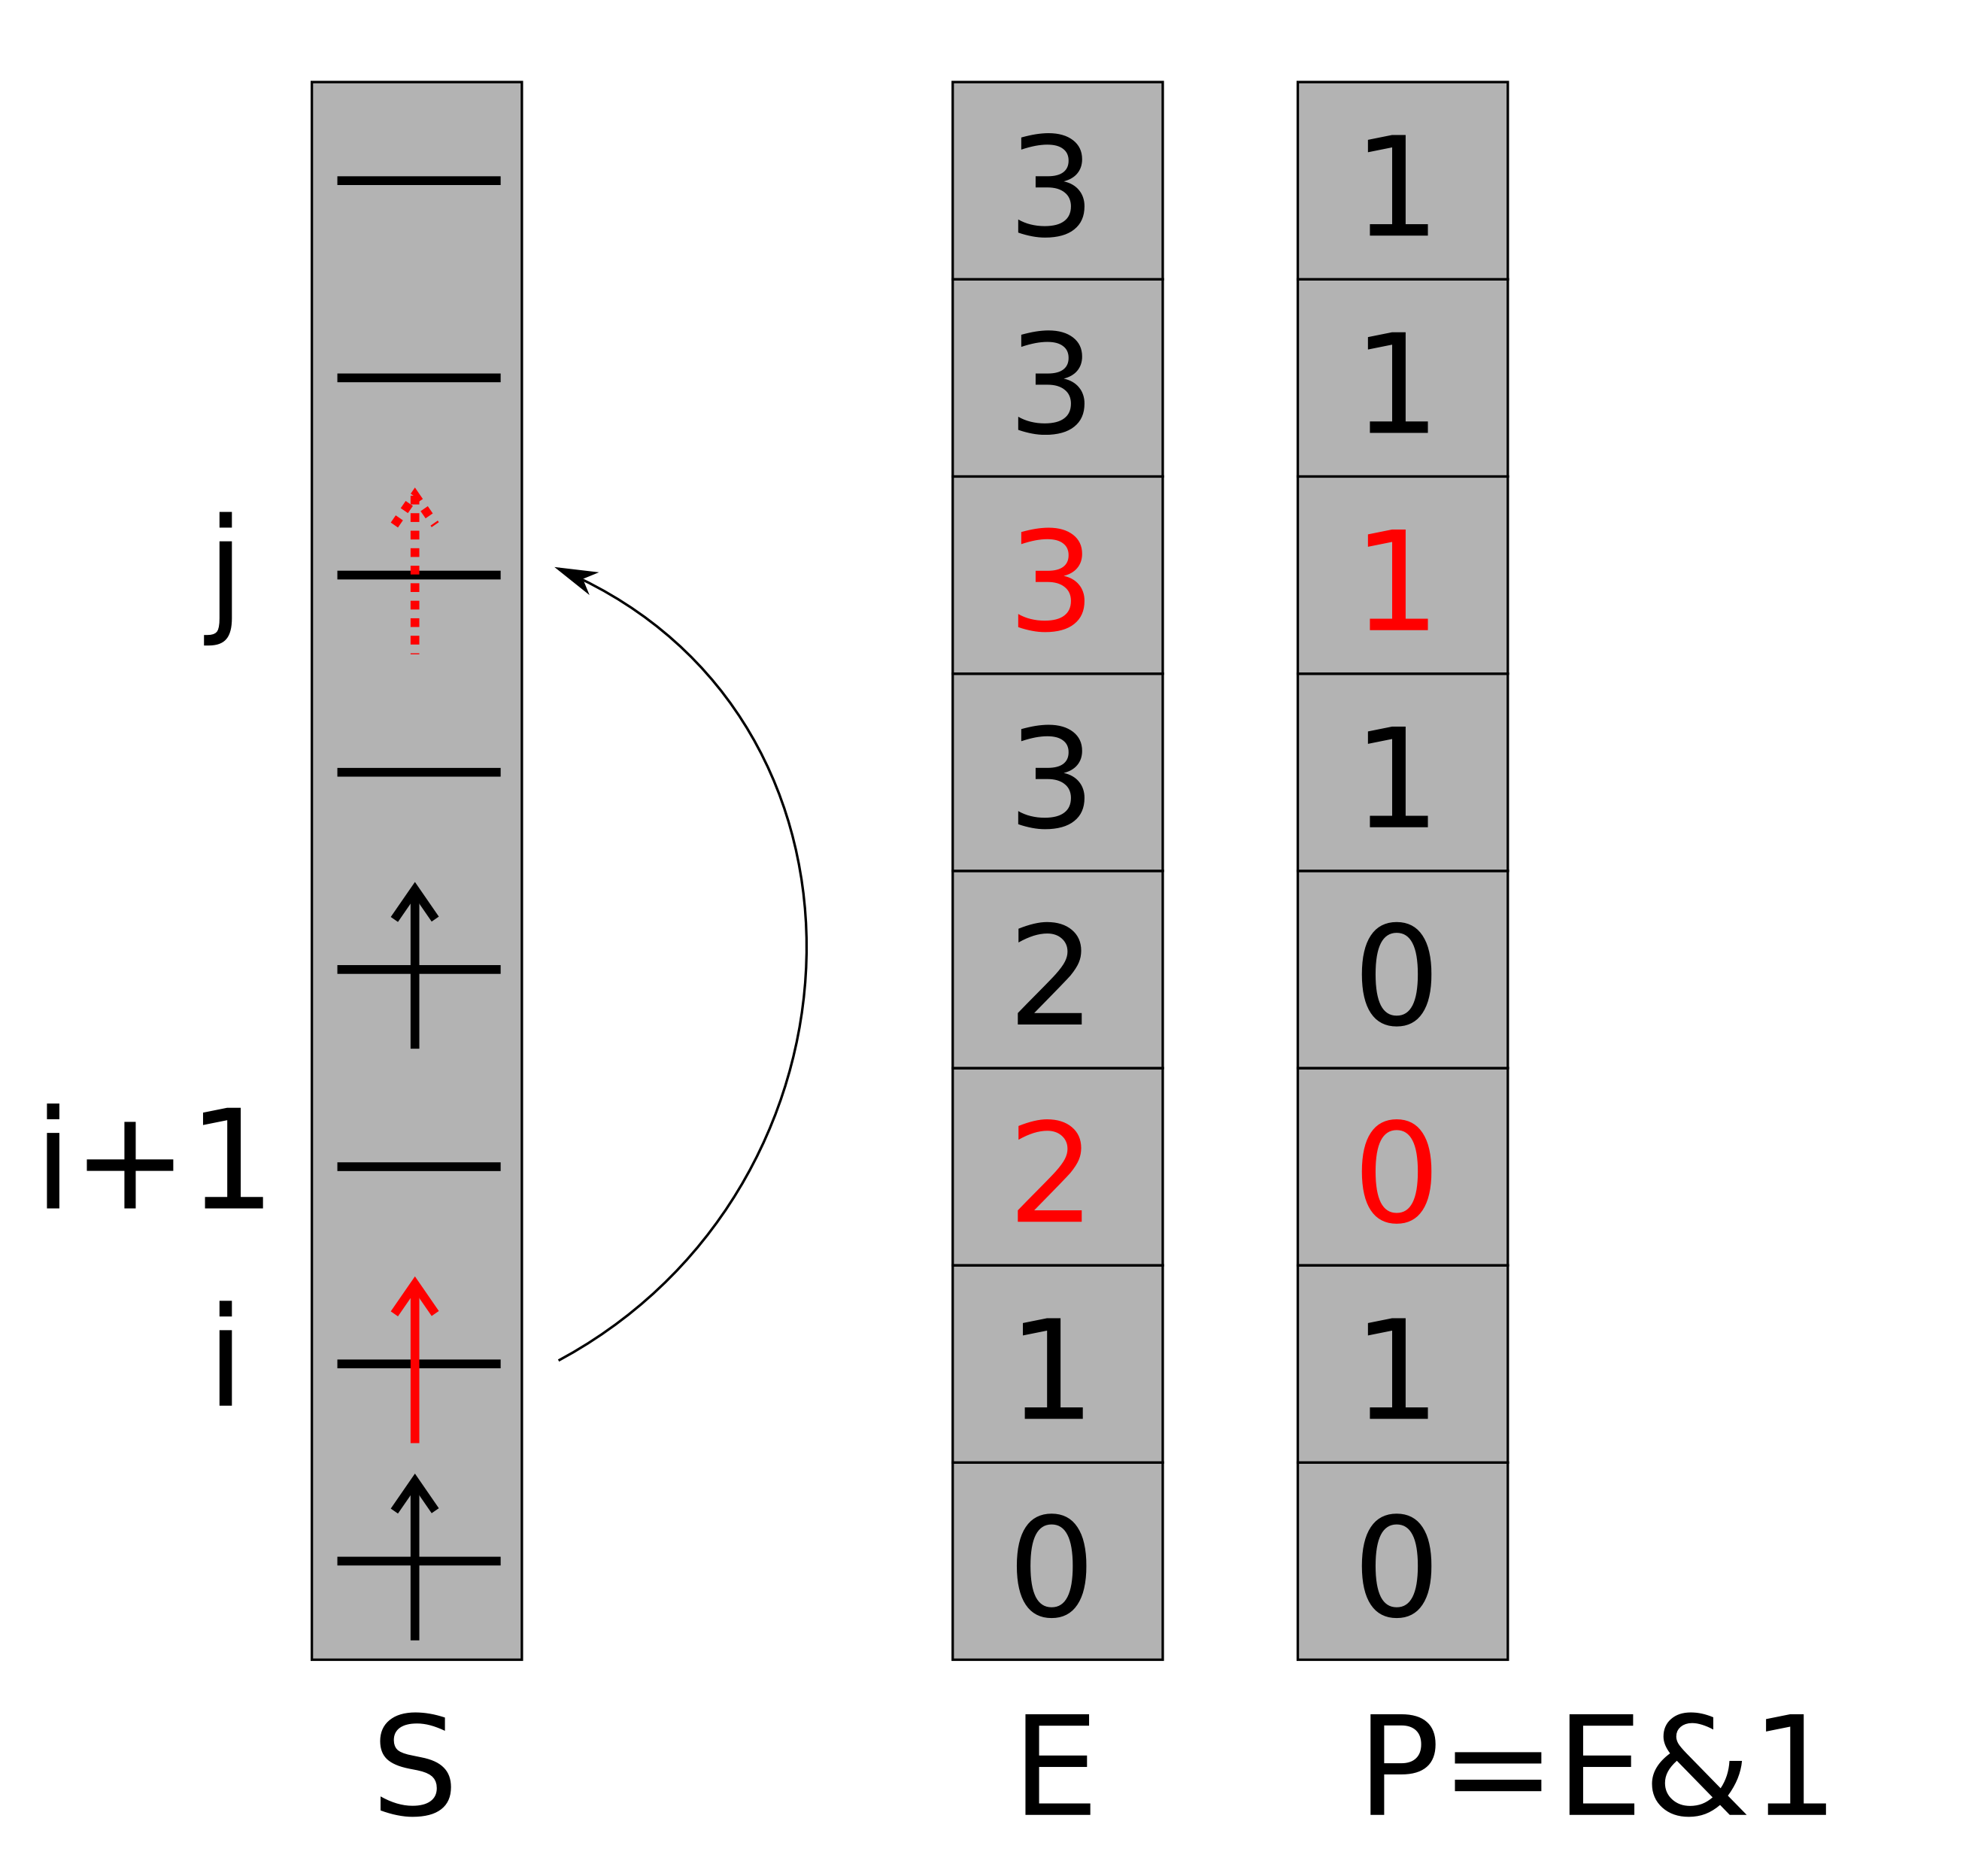
\includegraphics[width=0.6\columnwidth]{figures/determinant_driven/phase}
		\caption{
		\label{generators_selectors}%
		phasemask
		}
		commentt
	\end{center}
\end{figure}
        
Currently, the quantum package does not store the $P$ vector for each variational determinant, but re-computes it whenever needed before a loop. The memory cost being negligible this way, for CPU performance reason, each bit is stored on a separate 32-bit integer.
The algorithm for computing $P^S$ is show as algorithm \ref{alg:PHASEMASK}. 
With this method, the cost of computing a phase - after paying the overhead of computing $P$ - is accessing two integers and IEOR them together (and tests.......). Unlike the general method, its cost doesn't depend on $\Nint$, and doesn't require to deal with the boundaries of 64-bit integers which are ANNOYING AS FUCK.
        

\subsection{Biexcitation}







A double excitation is a product of two single excitations.
In the case of an $\alpha \beta$ double excitation, the two single excitations are independant, so the phase factor is merely the product of the phase factors computed for each spin part. 


$$phase(\hat T_{p \bar q}^{r \bar s}, \ket I) = phase(\hat T_{p}^{r}, \ket I) \times phase(\hat T_{ \bar q}^{ \bar s}, \ket I) $$

There is a slight complication for $\alpha \alpha$ or $\beta \beta$ excitations.

As far as phase computation goes, it is irrelevant which index of an exciation operator is a creaion and which is an anihilation. So, for convenience, we can write single excitations without defining it

$$\tilde T_{ab} \in \{\hat T_a^b, \hat T_b^a \}$$

Considering a double excitation $\hat T^2$ involving 4 spinorbitals $p,q,r,s$ of same spin, there are two possible situations, shown in figure \ref{fig:biphasefactor}. 

%$$\hat T^2 = \hat T_{pr} \hat T_{qs}$$
%$$\hat T_{pr} \in \{ T_p^r, T_r^p\} ; p<r; \hat T_{qs} \in \{ T_q^s, T_s^q\};q<s$$ 

\begin{itemize}
\item
It can be expressed as two single excitations that do not cross, i.e.
$$\hat T^2=\tilde T_{pr} \tilde T_{qs};p<r<q<s$$
In this case, the numbers of particles in the ranges $]p, r[$ and $]q, s[$ remain unchanged, so we can write
$$phase(\hat T^2, \ket I) = phase(\tilde T_{pr}, \ket I) \times phase(\tilde T_{qs}, \ket I) $$

\item
It can be expressed as two single excitations that cross, i.e.
$$\hat T^2=\tilde T_{pr} \tilde T_{qs};p<q<r<s$$
As we can see in figure \ref{fig:biphasefactor}, applying  $\tilde T_{qs}$ results in a particle being created or anihilated in the range $]p,r[$, resulting in a change of parity for the number of particles in that range. Therefore
$$phase(\tilde T_{pr}, \tilde T_{qs} \ket I) = -phase(\tilde T_{pr}, \ket I)$$ 
$$phase(\hat T^2, \ket I) = -phase(\tilde T_{pr}, \ket I) \times phase(\tilde T_{ qs}, \ket I) $$
\end{itemize}



\begin{figure}[h!]
	\begin{center}
		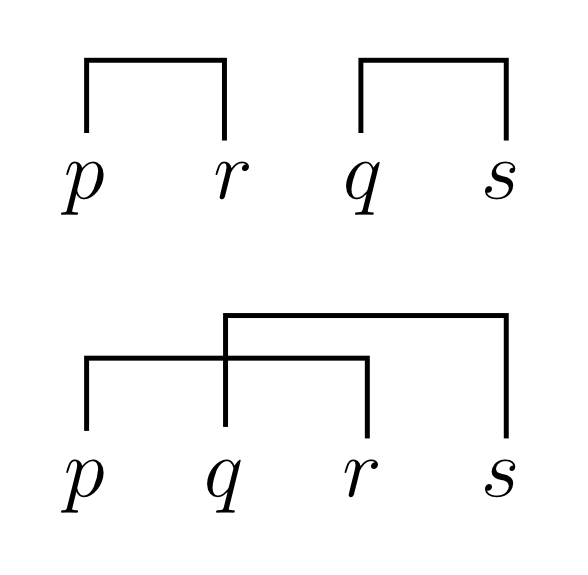
\includegraphics[width=0.4\columnwidth]{figures/determinant_driven/biphasefactor}
		\caption{
		\label{fig:biphasefactor}%
		phasemask
		}
		commentt
	\end{center}
\end{figure}

%extra permut si:
%$[(p-r) \oplus (p-s)] \vee [(q-r) \oplus (q-s)] > 0$


\section{integrals}
hashtable \\

\section{generating a subspace}
duplicates are avoided by checking connection to the past \\
******** (ptet exemple avec generator\_CAS versus generator\_full PSI is filtered with different function and supplied to the module using cas\_sd ( cas\_sd, mrcc ) or full\_ci ( pt2 stoch ) )?? \\
================

Generally speaking, a subspace is defined by a reference and a class of excitation applied to it. Because of the determinant-driven approach, it may not be possible to store all the determinants of the considered subspace. 

% - as a matter of fact there is no algorithm to systematically generate all determinants for a defined subspace. The idea to 


\paragraph{reference}

The quantum package allows to define either a CAS or the full-CI as the reference ( although the full-CI is a particular CAS, it is treated differently at the code level ).

\paragraph{excitation class}
The excitations to be applied to the reference are defined by 6 sets of spinorbitals
\begin{itemize}
\item
Holes and particles allowed for single excitations (2 sets)
\item
Holes and particles allowed for the first of a double excitation (2 sets)
\item
Holes and particles allowed for the second of a double excitation (2 sets)
\end{itemize}

This allows to accurately define a subspace. Typically, to define a CAS-SD

\begin{itemize}
\item
\emph{core orbitals} : part of no sets
\item
\emph{inactive orbitals} : part of all "hole" sets
\item
\emph{active orbitals} : part of all sets
\item
\emph{virtual orbitals} : part of all "particle" sets
\item
\emph{deleted orbitals} : part of no set
\end{itemize}


 As will be seen later, determinants are selected iteratively. The general procedure is shown 



\begin{algorithm}
	\caption{GENERAL\_SELECTION}	
	\label{alg:GENERAL_SELECTION}	
	$\ket {\Psi} \gets \ket {HF}$\;
	add CAS spinorbitals to $H_0, H_1, H_2, P_0, P_1, P_2$ \;
	$\hat T$ the list of excitations allowed on the reference based on $H_0, H_1, H_2, P_0, P_1, P_2$ \;
	
	\While{some condition}{
		$C$ the list of determinants of $\Psi$ that are part of the CAS reference \;
		\ForAll{$C_i \in C$}{
			\ForAll{$T_j \in T ; T_j \ket {C_i} \neq 0$}{
				$\ket \alpha \gets T_j \ket {C_i}$ \;
				\If{$not(T_k \ket {C_{l<j}} = \ket \alpha) \&\ Selection\_criterion$}{
					add $\ket \alpha$ to $\Psi '$ \;			
				}
			}
		}
		do some selection in $\Psi'$ \;
		add selected determinants to $\Psi$ \;
		diagonalize $\Psi$ \;
	}
\end{algorithm}

\end{document}
